\section*{Тренировочное задание}

В соответствии с \textbf{вариантом 1} необходимо:
\begin{enumerate}
    \item дополнить временной план проекта, подготовленный на предыдущем этапе
(лабораторная работа № 1), информацией о ресурсах и определить стоимость
проекта.
    \item для этого заполнить ресурсный лист в программе MS Project, принимая во
внимание, что к реализации проекта привлекается не более 11 человек.
    \item предусмотреть, что стандартная ставка ресурса составляет 120 руб./день.
    \item произвести назначение ресурсов на задачи в соответствии с таблицей~\ref{tbl:t_1}. С учетом
того, что квалификация ресурсов одинаковая, при назначении ресурсов
использовать процент загрузки.
    \item на 3-й день реализации работы В арендуется оборудование по ставке 5 тыс. руб.
в неделю. На его установку и наладку необходимо выделить 2 тыс. рублей.
\end{enumerate}

\captionsetup{justification=raggedright,singlelinecheck=off}
\begin{table}[h]
    \caption{\label{tbl:t_1}Временные характеристики проекта}
    \begin{center}
        \begin{tabular}{|c|c|}
                    \hline
              \textbf{Название работы} & \textbf{Количество исполнителей (чел.)}            \\ \hline
            Работа A  & 2    \\ \hline
            Работа B & 6    \\ \hline
            Работа C  & 2    \\ \hline
            Работа D  & 5    \\ \hline
            Работа E  & 4    \\ \hline
            Работа F  & 6    \\ \hline
            Работа G  & 1    \\ \hline
            Работа H  & 7    \\ \hline
            Работа I  & 1    \\ \hline
            Работа J  & 4    \\ \hline
            \end{tabular}
    \end{center}
\end{table}

\subsection*{Результат}


\begin{figure}[h!]
	\begin{center}
		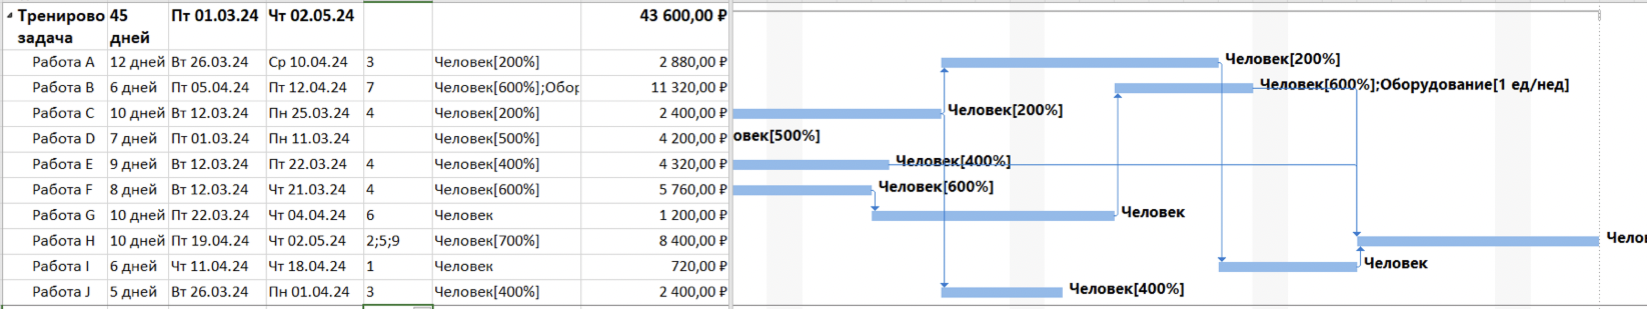
\includegraphics[scale=0.28]{inc/img/p_1.png}
	\end{center}
	% \captionsetup{justification=centering}
	% \caption{Параметры рабочей среды}
	\label{fig:u1}
\end{figure}

Наблюдается перегрузка ресурса.

\begin{figure}[h!]
	\begin{center}
		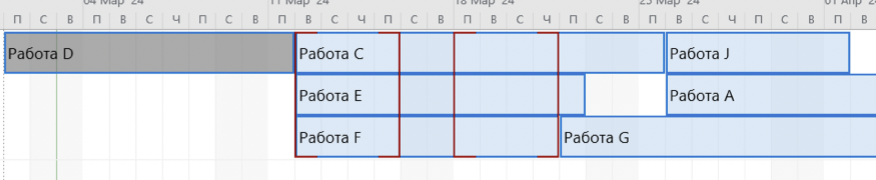
\includegraphics[scale=0.45]{inc/img/p_2.png}
	\end{center}
	% \captionsetup{justification=centering}
	% \caption{Параметры рабочей среды}
	\label{fig:u1}
\end{figure}


\section*{Лабораторная работа}

\subsection*{Задание 1: создание списка ресурсов}

Был заполнен ресурсный лист в соответствии с таблицей:

\begin{figure}[h!]
	\begin{center}
		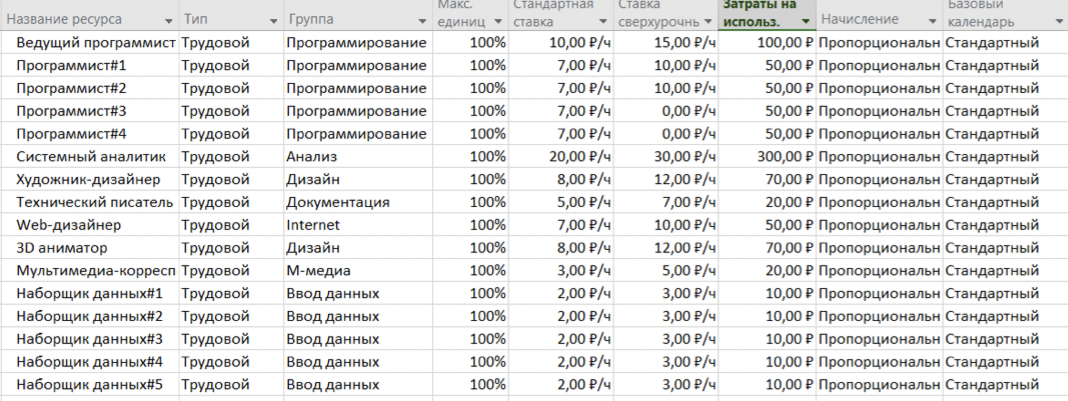
\includegraphics[scale=0.45]{inc/img/p_3.png}
	\end{center}
	\captionsetup{justification=centering}
	\caption{Ресурсный лист}
	\label{fig:u3}
\end{figure}

\subsection*{Задание 2: назначение ресурсов задачам}

Были назначены ресурсы задачам в соответствии с таблицей; задачам 2, 8, 12
было выделено по 1000 рублей фиксированных затрат; для 8 задачи
«Построение базы объектов» был арендован дополнительный сервер со
стоимостью аренды 2 рубля в час:

\begin{figure}[h!]
	\begin{center}
		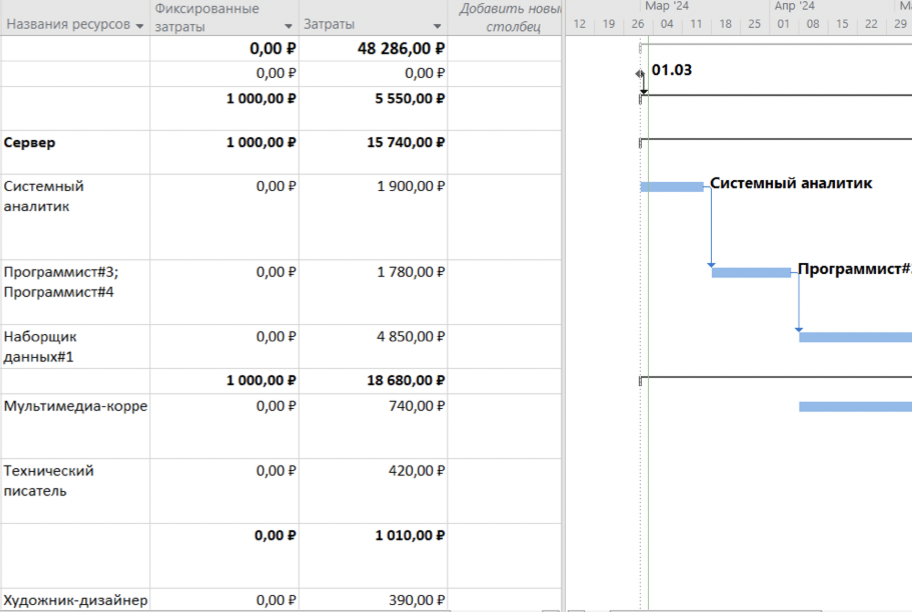
\includegraphics[scale=0.5]{inc/img/p_4.png}
	\end{center}
	\captionsetup{justification=centering}
	\caption{Назначение ресурсов задачам}
	\label{fig:u3}
\end{figure}

У системного аналитика, художника-дизайнера и технического писателя
имеется перегрузка из-за наложения задач.

\begin{figure}[h!]
	\begin{center}
		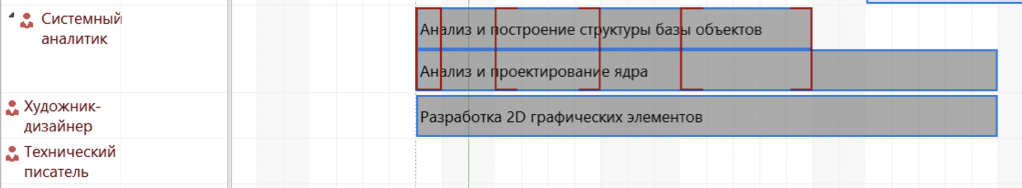
\includegraphics[scale=0.4]{inc/img/p_5.png}
	\end{center}
	\captionsetup{justification=centering}
	\caption{Перегрузка из-за наложения задач}
	\label{fig:u3}
\end{figure}

\begin{figure}[h!]
	\begin{center}
		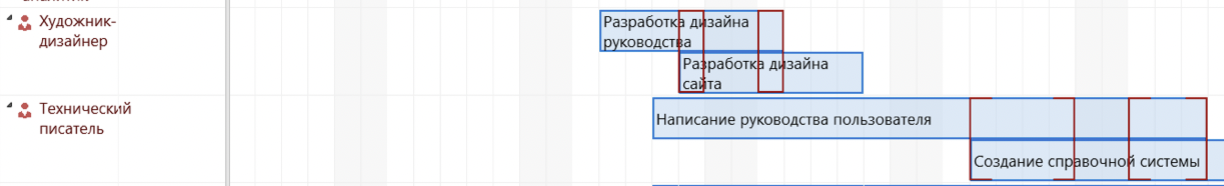
\includegraphics[scale=0.35]{inc/img/p_6.png}
	\end{center}
	\captionsetup{justification=centering}
	\caption{Перегрузка из-за наложения задач}
	\label{fig:u3}
\end{figure}


\newpage

\subsection*{Задание 3: анализ затрат по группам ресурсов}

Была проведена структуризация затрат по группам ресурсов:

\begin{figure}[h!]
	\begin{center}
		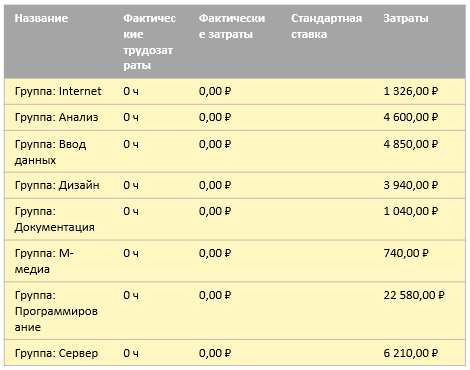
\includegraphics[scale=0.9]{inc/img/p_8.jpg}
	\end{center}
	\captionsetup{justification=centering}
	\caption{Анализ затрат по группам ресурсов}
	\label{fig:u3}
\end{figure}

\begin{figure}[h!]
	\begin{center}
		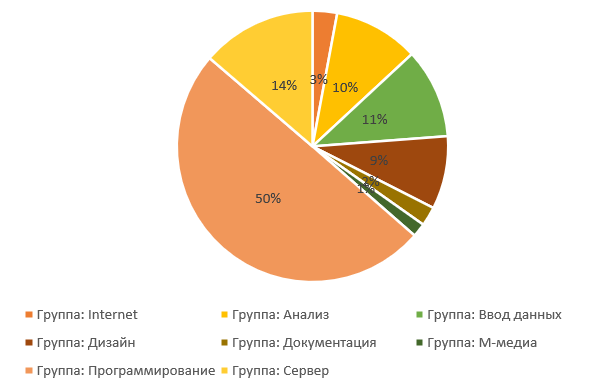
\includegraphics[scale=0.92]{inc/img/p_7.png}
	\end{center}
	\captionsetup{justification=centering}
	\caption{Анализ затрат по группам ресурсов}
	\label{fig:u3}
\end{figure}

Информация о затратах и трудозатратах по структурным группам ресурсов
представлена в графическом виде.

\begin{figure}[h!]
	\begin{center}
		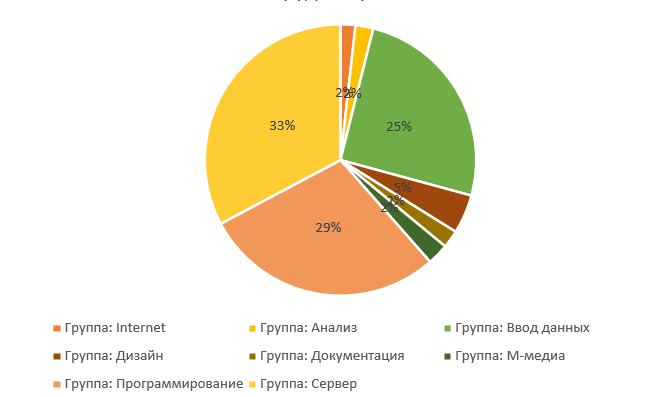
\includegraphics[scale=0.92]{inc/img/p_9.jpg}
	\end{center}
	\captionsetup{justification=centering}
	\caption{Анализ трудозатрат по группам ресурсов}
	\label{fig:u15}
\end{figure}

\clearpage

При сопоставлении в логике «Деньги» --- «Объем работ» («Затраты ---
Трудозатраты»), можно сделать следующие выводы.
\begin{itemize}
    \item[---] Наибольшие денежные затраты уходят на группы Программирование,
Сервер, Ввод данных и Анализ.
    \item[---] Наибольший объем работ – у групп Сервер, Программирование
и Ввод данных.
    \item[---] Трудозатраты на группы Программирование, Ввод данных и
Документация примерно равны, но отношение затрат – сильно
различается: 50, 11 и 14 процентов, соответственно.
    \item[---] Наибольшее отношение затрат к трудозатратам – у группы Анализ (10
процентов к 2), наименьшее – у группы Сервер (14 к 33), равно
примерно единице – у групп Internet, Документация и Медиа.
\end{itemize}


\subsection*{Статистика по проекту}

На рисунке~\ref{fig:u20} представлены данные о затратах проекта, а также о его длительности.

\begin{figure}[h!]
	\begin{center}
		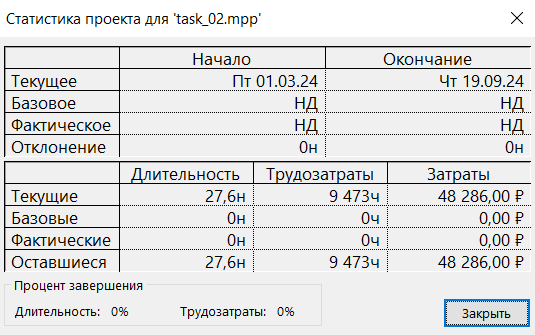
\includegraphics[scale=0.92]{inc/img/p_10.jpg}
	\end{center}
	\captionsetup{justification=centering}
	\caption{Статистика по проекту}
	\label{fig:u20}
\end{figure}

\subsection*{Вывод}

В ходе выполнения лабораторной работы были изучены возможности
программы Microsoft Project для работы с ресурсами. Была заполнена таблица
ресурсов, затем ресурсы были назначены задачам, проведён анализ затрат и
трудозатрат по группам ресурсов.

Итоговые затраты проекта --- 48 286 руб, длительность 27,6 недель. Проект укладывается в рамки бюджета (50 000  руб) и не
укладывается в даты (6 месяцев).

Некоторые сотрудники перегружены из-за наложения задач. Необходимо
пересмотреть планирование этих задач. Соотношение затрат и трудозатрат в
некоторых категориях крайне непропорционально.

